\documentclass{article}
\usepackage[T1]{fontenc}
\usepackage[utf8]{inputenc}
\usepackage{amsfonts}
\usepackage{amssymb}
\usepackage{amsmath}
\usepackage{graphicx}
\usepackage{url}
\usepackage{float}
\usepackage{hyperref}
\hypersetup{%
    pdfborder = {0 0 0}
}
\usepackage{tabularx}
\usepackage{verbatimbox}
\usepackage{color, colortbl}
\usepackage{booktabs}
\usepackage[
backend=biber,
style=numeric,
]{biblatex}

\addbibresource{bibliography.bib}

\definecolor{LightSteelBlue}{rgb}{0.69,0.77,0.9}

%\author{Hjalti Leifsson (hjaltil13@ru.is)\\Jóhann Örn Bjarkason (johannob01@ru.is)}
%\title{
%	\textbf{\huge{Project Discovery}} \\
%	\large{Advancing scientific research by implementing citizen science in EVE Online}
%}
\begin{document}
%\maketitle
 \newcommand{\HRule}{\rule{\linewidth}{0.5mm}}
\begin{titlepage}

\begin{center}
% Upper part of the page

\includegraphics[width=0.55\textwidth]{./rulogo}\\[4.0cm]    

%\textsc{\LARGE Háskólinn í Reykjavík}\\[1.5cm]

\textsc{\LARGE Final Project}\\[0.5cm]
%\textsc{\Large Dæmatímaverkefni 8}\\[0.6cm]

% Title
\HRule \\[0.4cm]
{ \Huge \bfseries Work Schedule and Procedures}\\[0.4cm]

\HRule \\[1.5cm]


% Author and supervisor
\begin{minipage}{0.49\textwidth}
\begin{flushleft} \large
\emph{Students:}\\
Hjalti Leifsson \\
Jóhann Örn Bjarkason
\end{flushleft}
\end{minipage}
\begin{minipage}{0.49\textwidth}
\begin{flushright} \large
\emph{Teachers:} \\
Hallgrímur Arnalds \\
Hannes Pétursson \\
Hlynur Sigurþórsson
\end{flushright}
\end{minipage}

\vfill

% Bottom of the page
{\large \today}



\end{center}

\end{titlepage}
\tableofcontents
\section{Introduction}\label{sec:introduction}

In this report we discuss the progress of our final project, \emph{Project Discovery}. In section~\ref{sec:time} we list the hours we have spent so far on the project in total and for each of us. In section~\ref{sec:burndown} we show the status of the burndown chart at this point, after four sprints have been completed. In section~\ref{sec:backlog} we go over the sprint backlogs of the sprints we've done so far and show the burndown charts for each sprint we have completed. Lastly in section~\ref{sec:retrospectives} we summarize our sprint planning and retrospective meetings. 
\section{Background}\label{sec:background}
	In this section we discuss what a game with a purpose is, why our project falls within that category, we name the affiliates to this project, and what they have done for the project. Finally, we outline the previous work already committed to the project by previous students, and where we picked up the project.

\subsection{Game with a purpose}
	In the modern world it is one of the facts of life that people play video games, either competitively or casually, and the hours humans spend each year on video games is in the billions. If we could channel some of that time and energy into something really useful, we could do some amazing things, like solving large scale, real world scientific problems.

	Many scientific research projects require the analysis and/or classification of huge amounts of data, in these cases, the few scientists on the projects can not conceivably process the data themselves in their lifetime. One might think we could use computers to solve such problems for us automatically, but despite colossal advances over the last 50 years, computers still don't possess many skills and capabilities that most humans take for granted, such as perceiving an image and discern its patterns.

	Because humans possess complex conceptual intelligence, perceptual capabilities and pattern recognition that modern algorithms and machine learning can not yet mimic, computers can not be used to solve these problems for us; human interaction is needed. If we could use a large number of ordinary humans as biological processors in a distributed computer-like system, we could solve real world large scale problems that would otherwise be considered impossible or too time consuming.

	Seeing how popular video games are, what if we designed a game whose purpose is outsourcing computationally difficult functions to humans in an entertaining way? These \emph{games with a purpose} are an implementation of citizen science and ways for regular people outside the scientific community to contribute to scientific research in various fields, and entertaining themselves in the meantime.

	This concept of using games for citizen science has already been proven useful before in games such as \emph{FoldIt}, where players compete to find the lowest energy state of a protein, thus helping research in the prediction of protein structures, and \emph{Galaxy Zoo}, where players help each other classifying astral bodies in order to find out how galaxies are formed.

	The goal of this project is creating such a \emph{game with a purpose}, utilizing citizen science, where ordinary people can play a game for fun and solve real world scientific problems in the meantime.

	% TODO: Insert references to https://www.cs.cmu.edu/~biglou/ieee-gwap.pdf

\subsection{Human Protein Atlas}

	This project aims to finish analyzing and classifying the images in one subpart of the The Human Protein Atlas (HPA), the Subcellular Atlas.

	The Subcellular Atlas contains around five hundred thousand, high resolution, multicolor images of immunofluorescently stained cells that reveal spatial expression patterns at the subcellular level. Around half of those images have already been classified by scientists at the HPA the past few years, and by way of citizen science, we can classify the rest of these images much faster, freeing up the time of these scientists.

	The HPA is a scientific program based in Sweden, and is funded by the Knut and Wallenberg foundation in order to allow for a systematic exploration of the human proteome using antibody-based proteomics. The HPA contains information for a large majority of all human protein-coding genes regarding the expression and localization of the corresponding proteins based on both RNA and protein data.

	The HPA consists of four subparts: normal tissue, cancer, subcellular and cell lines with each subpart containing images and data based on antibody-based proteomics and transcriptomics.

	If this project succeeds, the HPA can provide a better database of images to scientists around the world, since the database is open to researchers anywhere to use. This can have drastic improvements in the fields of biological research, and really helps in understanding how diseases such as cancer operate, which in turn helps in the way of finding a cure. 

	Moreover, if this project succeeds with an acceptable accuracy, the same method can be used on other parts of the HPA, in fact, this whole project has been designed with that in mind, to ease the transition into classifying different kinds of data. 

	% Cite HPA website http://www.proteinatlas.org/

\subsection{MMOS}

	Massively Multiplayer Online Science (MMOS), the name of the concept, and the name of the Swiss company behind it, challenges the way that citizen science is carried out today. 

	While current citizen science projects either create entire new games or "gamify" menial tasks for each research project, the MMOS method is to inject research projects into existing, popular games as seamless parts of their gaming experience (including mechanics, narrative, and visuals). With the MMOS method, we can benefit from the time that players already spend on the already existing games. Even if we can only direct a small fraction of this time to scientific projects, we can provide a huge network of human volunteers to scientific research.

	For this project, MMOS provided an API, which served as a thin interface between the scientific research data from the Human Protein Atlas and the MMORPG EVE Online. It took care of everything related to the citizen science problems, such as task allocation to players, tracking and scoring player performance, giving feedback to the Project Discovery reward system and aggregating results for scientific research. This interface made it easier for us to integrate Project Discovery into EVE Online, since we could focus on coding the client itself into EVE Online. This also substiantially lowered the entry barrier for CCP to implement this feature.

	The MMOS method addresses the core challenges of citizen science games for the following reasons:

	\begin{itemize}
	  \item {\bf Engagement:} There is a massive amount of user base already engaged, motivated to solve complex tasks.
	  \item {\bf Motivation \& Retention:} As the solution is not a secret to the gamer, the intrinsic motivation of helping science is very important, but to keep up the long-term engagement, integrating it with in-game reward systems and other game mechanics is vital and adds an additional layer of motivation.
	  \item {\bf Separation of Concerns:} Researchers do their research work (defining tasks, analyzing results, communicating in research related issues) and professional game designers create the in-game experiences.
	  \item {\bf Reliability:} Popular, massively multi-player games tend to last for many years, with some running for more than a decade with hundreds of thousands of devoted players.
	\end{itemize}

	We believe that this approach offers a win-win situation that benefits all parties: scientists, game players, and the gaming industry at large.

	% Cite the paper from david thue

\subsection{CCP Games and EVE Online}

	CCP Games is an Icelandic video game developer and publisher which is best known for producing EVE Online, the player-driven science fiction space-MMORPG which is home to over 7,000 star systems and hundreds of thousands of players. CCP showed enthusiasm about this project and was willing to see if the EVE Online community showed positive reactions to helping real world science while in a science fiction environment. If so, CCP was willing to host this game fully on the EVE Online live servers where the whole EVE universe would be able to participate in the project.

	CCP Games allowed us access to two work stations within their headquarters in Reykjavík, and placed us in an EVE development team with senior EVE developers who were available to us when we needed help with the project. We were also allowed access to the cafeteria with complementary lunch, which allowed us to stay in house and focus on development.

	EVE Online was a good fit for this project, since EVE is a science fiction game set in space, a scientific project like this would not feel out of context to players. Especially since the subcellular atlas from the Human Protein Atlas was chosen especially because its images complement the theme of EVE and look stunning within the client. Furthermore, EVE Online players are used to getting pretty technical and difficult tasks in game already, such as the hacking mini-game. EVE Online's gameplay is also well suited to mini-games of this sort since there are periods in the game which players spend waiting and players could utilize those waiting periods to analyze a few images.

	In order to entice EVE players to play our \emph{game with a purpose}, we offer EVE Online currency for each task solved. That way the game offers the players something that is already of value to them, something that other citizen science games were unable to do, since the rewards are usually only based within the game itself.

\subsection{Previous work}
	This project was a continuation of work done by Reykjavík University graduates Gunnar Þór Stefánsson and Þór Adam Rúnarsson. They worked on it as their final project for the spring semester of 2015 in collaboration with the same companies as we did for this project.

	They created a web prototype very quickly which allowed for basic functionality with a connection to the MMOS API. This prototype was showcased at EVE Fanfest 2015 and was very well received by EVE Online players and CCP alike, which is why they decided to start integrating the prototype into the EVE Online client immediately. They used their remaining time for the semester to focus on integrating the client into EVE Online, and managed to create a crude version of the game before the semesters end.

	They continued their work on the client during the summer of 2015 with a research grant from Rannís, The Icelandic Center for Research. In the beginning of July, Gunnar Þór Stefánsson left the project, and Hjalti Leifsson replaced him. The work continued until Þór Adam Rúnarsson left the project and Jóhann Örn Bjarkason joined in the end of August, when Reykjavík University offered to continue the project as a Final Project.

	When we started the project, the game itself was at a prototype stage. The user interface had a hexagonal category selection as well as header and footer elements according to the current design. The game was able to connect to the MMOS API using HMAC-SHA256 authentication, receive new tasks and submit classifications. A simple rewarding system was already in place, rewarding players with in game currency (ISK), experience points (XP) and loyalty points (LP) when players submitted a solution. When the client received a response from the API, it calculated the appropriate rewards, and displayed a rewarding screen. Finally, a rudimentary tooltip based tutorial phase was implemented, which explained the interface to the user. Nothing else was implemented at that point in time, and that is where we started work on the project, implementing the remaining features according to design with help from CCP Games and MMOS.

	%Hvar nefnum við það sem við gerðum?
\section{Project Discovery}\label{sec:projectdiscovery}

\subsection{Network Communications}

\subsection{Architecture}

\subsection{Client within a client}

\subsection{Game logic}

\subsection{The science behind the game}

\subsection{The website}
One of the goals of the project was to launch a Project Discovery website along with the release of the game. The website serves as an information hub for the project. Interested parties can get information about the game, the science behind the game and our partners, MMOS and the Human Protein Atlas. The website also displays videos related to the game and screenshots of the game in action. To build the website we used HTML5, Less and JavaScript. We were provided with a template from web developers within CCP which helped us make the website look 
\section{User evaluation}\label{sec:userevaluation}

We performed a preliminary, in-house user evaluation in early October. This was not a part of the original project description but we were advised by Pétur Örn Þórarinsson, our project manager, to do this before the \emph{Project Discovery} game would be showcased at EVE Vegas~\cite{vegas}, a conference for \emph{EVE Online} players and fans. The purpose of this test was to shed light on any obvious errors with the game, especially the tutorial phase which was at an early stage at the time.

\subsection{Implementation}
The tests took place on the 9th of October 2015. We got five participants from CCP, four males and one female between the ages of 25 to 40. The people were a mix of game designers, quality assurance people and community developers. The reason we only got people from within CCP to partake in the tests was that the game was not ready to be revealed to the public so we could not get people outside of CCP to take part.

The test was performed on a computer that remotely connected to our personal work desktop. The evaluation was performed as follows, a participant arrived, we greeted them, thanked them for coming, and explained the procedure. The procedure was that the participant would sit down and we would observe them while they played \emph{Project Discovery}. The participant would open \emph{Project Discovery}, finish the tutorial and a handful of other tasks. While playing, we asked the participant to think aloud. Participants could play for as long as they wanted within a reasonable amount of time, given that they continued to think aloud.

After the participant had finished playing we asked them questions about their experience playing the game and then thanked them for their contribution to the project. The questions we asked participants and their answers can be found in appendix \ref{sec.data}.

\subsection{Results}

In this section we analyze the data we derived from the tests and how we used that data to improve the game.

\subsubsection{Tool-tips}
We gathered that proper use of tool-tips was paramount to the players understanding of the game. Some players seemed to be confused about the objectives of the game. We saw that the tool-tips needed to be clear and helpful to the players understanding the interface. So we decided that tool-tips should be utilized when the players first see the interface, and also throughout the whole tutorial and training session, gradually teaching players about the game as they face the actual problems. The tool-tips also needed to be shorter and focused on one specific message. Participants did not immediately grasp that they could change the color filter on the main image, so we added a tool-tip that describes this functionality.

\subsubsection{Tutorial}
Participants felt that the tutorial was too easy and did not teach them very much about the real game. To rectify this we implemented a more extensive tutorial, where each task teaches the player a specific aspect of the game, such as explaining the interface, or how to classify certain patterns in images. 

Participants expressed the need for an explanation after each tutorial task, so we reached out to the researchers at the HPA to get explanations for each training task, and to explain why the correct solution was correct. We also enlisted their help in making the tutorial more focused and better at teaching players the skills needed to classify images.

\subsubsection{Interface}
Participants did not have much to say about the interface with the exception of everyone being in agreement that a magnification function was necessary on the main image. We responded to that by implementing a magnification function that allows players to zoom in to the full resolution of the main image within the image container and it gives players the option to fix the position of the zoomed in image so they can easily compare the image to the categories available.

We observed that participants, who had completed the training phase, and were contributing to unknown tasks, did not get a result screen. That is normal behavior since the solution is unknown, we can not reliably give a result. We saw that when users weren't getting instant feedback they were not as interested and seemed less motivated to find the right solution to the tasks. Our solution to this problem was that since we do know the community consensus for specific tasks at any given time, we can show exact percentages for choices by other players. 

We felt that since participants expressed excitement in seeing a result screen, we should implement this for unknown tasks, so that the game would not lose the factor of excitement once players reach the stage of solving images that have no known solution. To achieve this, instead of giving players a confirmed correct answer like we do with training tasks, we give players the current consensus of the task at the time the user submitted his solution. This consensus screen can be seen in figure \ref{fig:consensus}. We also make sure to let players know that this consensus is not necessarily correct. That way the player can get a sense of what other players think the solution is and can see if he is in agreement with them or not.

\begin{figure}[H]
	\centering
	\graphicspath{ {./graphics/} }
	\centerline{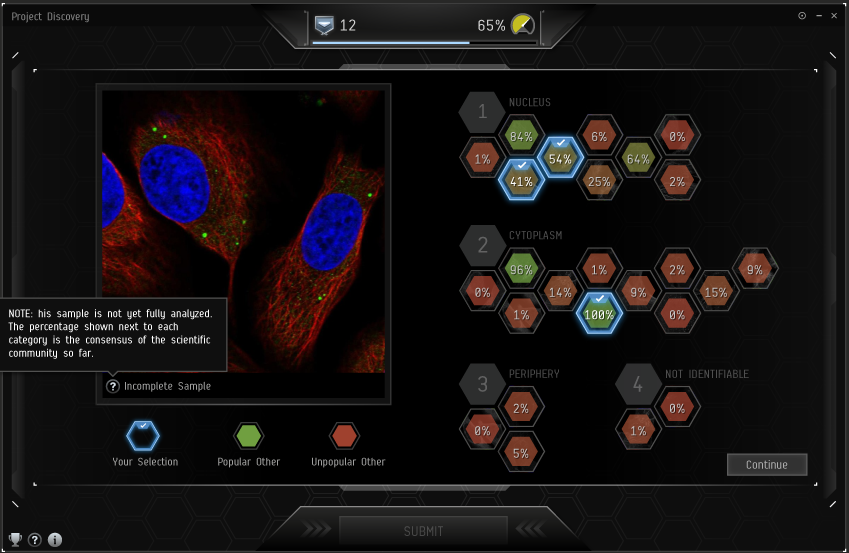
\includegraphics[scale=0.55]{unknown_result.png}}
	\caption{\label{fig:consensus}A mock-up of the consensus screen for unknown tasks.}
\end{figure}

\subsection{Conclusion}
	The user evaluation proved to be very advantageous for us. It gave us great ideas to improve the game which we would probably not have thought of otherwise, since it was impossible for us to experience the game as new players. The participants were overall very positive about the game, four out five played it for longer than we asked them to, because they enjoyed solving the tasks. A majority of the players took great care in solving the tasks by paying close attention to everything. All but one participant expressed interest in playing the finished version of the game.


\section{Work schedule and flow}\label{sec:workscheduleandflow}

In this section we will discuss the work schedule we put together and how we managed to follow that schedule. We will also go into the methodology we decided to use to aid us during the project and how that influenced the project. As a part of that we will show the burndown chart for the project as a whole and discuss all of the sprints that we finished while working on the project.

\subsection{Initial plan}

Our work schedule was split into two different phases. The first was during the 12 week semester from the 17th of August to November the 11th. Our schedule during that period was influenced by classes and course work in other courses. During the 3 week semester from the 26th of November to December the 16th this project was our only concern so we could dedicate most of our time to it. 

\subsubsection{Schedule for the 12 week semester}
  This table gives a detailed view of the hours we scheduled to work on the project during the 12 week term. This was the minimum amount of hours we pledged to dedicate to the project during the term. The difference in hours spent on the project for team members during this phase can be explained by a more favorable schedule in other courses for Jóhann. 

  \noindent
  \addvbuffer[12pt 12pt]{\begin{tabular} {| r | c | c | c | c | c | c | c |}
    \rowcolor{LightSteelBlue}
    \hline  & Mon & Tue & Wed & Thu & Fri & Sat & Sun\\ 
    \hline Hjalti & 16:00-18:00 & 16:00-18:00 & - & 12:00-15:30 & 10:00-14:00 & -  & - \\
    \hline  & - & - & - & - & 16:00-18:00 & - & - \\
    \hline Total & 2:00 & 2:00 & - & 3:30 & 6:00 & - & - \\
    \rowcolor{LightSteelBlue}
    \hline  &  Mon & Tue & Wed & Thu & Fri & Sat & Sun\\ 
    \hline Jóhann & 16:00-18:00 & 16:00-18:00 & - & 9:30-15:30 & 10:00-14:00 & -  & - \\
    \hline  & - & - & - & - & 16:00-18:00 & - & - \\
    \hline Total & 2:00 & 2:00 & - & 6:00 & 6:00 & - & - \\
    \hline
  \end{tabular}}

  \noindent This table sums up the total hours for the 12 week term.  
  
  \noindent
  \addvbuffer[12pt 12pt]{\begin{tabular} {| r |  c | c |}
  \hline & Hjalti & Jóhann\\
  \hline Total per week & 13.5 hours & 16 hours \\
  \hline Total for the semester & 162 hours & 192 hours \\
  \hline Total combined & \multicolumn{2}{c |}{354 hours} \\ 
  \hline
	
  \end{tabular}} 
  
\subsubsection{Schedule for the 3 week semester}
  This table shows the schedule for the 3 week term. The hours are the minimum commitment both team members made during this time.

  \noindent
  \addvbuffer[12pt 12pt]{\begin{tabular} {| r | c | c | c | c | c | c | c |}
    \rowcolor{LightSteelBlue}
    \hline  & Mon & Tue & Wed & Thu & Fri & Sat & Sun\\ 
    \hline Hjalti & 9:00-17:00 & 9:00-17:00 & 9:00-17:00 & 9:00-17:00 & 9:00-17:00 & 10:00-15:00  & 10:00-15:00 \\
    \hline Total & 8:00 & 8:00 & 8:00 & 8:00 & 8:00 & 5:00 & 5:00 \\
    \rowcolor{LightSteelBlue}
    \hline  &  Mon & Tue & Wed & Thu & Fri & Sat & Sun\\ 
    \hline Jóhann & 9:00-17:00 & 9:00-17:00 & 9:00-17:00 & 9:00-17:00 & 9:00-17:00 & 10:00-15:00  & 10:00-15:00 \\
    \hline Total & 8:00 & 8:00 & 8:00 & 8:00 & 8:00 & 5:00 & 5:00\\
    \hline
  \end{tabular}}

  \noindent This last table summarizes the total amount of hours we scheduled to spend on the project.
  
  \noindent
  \addvbuffer[12pt 12pt]{\begin{tabular} {| r |  c | c |}
  \hline & Hjalti &  Jóhann\\
  \hline Total per week & 50 hours & 50 hours \\
  \hline Total for the semester & 150 hours & 150 hours \\
  \hline Total for the previous semester & 162 hours & 192 hours \\
  \hline Total for the project & 312 hours & 342 hours \\
  \hline Total for the project combined & \multicolumn{2}{c |}{654 hours} \\ 
  \hline
  \end{tabular}}


\subsection{Methodology}
For this project we utilized the Scrum methodology to help us document and organize the project and its progress. The appointed Scrum Master was Jóhann, the Product Owner that represented the team was Hjalti and the Product Owner on behalf of CCP was Pétur Örn Þórarinsson who was also our Project Manager. Since the team only consisted of two people, the Scrum Master and Product Owner made up the the whole team. The project consisted of eight, two week long sprints, with the work divided so that the team could direct enough attention towards other courses, as well as work on the project.

Daily Scrum meetings were held at CCP headquarters every work day. During the three week term they took place at 11:30 AM, but they were held at various times of the day during the 12 week term, as the team wasn't always present throughout the day. We chose Scrum because it gave us good documentation on the team's progress and it gave us an indication of what we could achieve according to our velocity. With each iteration we could track what was going well and what needed improving. Scrum gave us the platform to review and improve on our process during each iteration.

\subsection{Progress during the project}

\subsubsection{Actual hours spent}

TODO: Insert images from toggl of hours spent once work is done.

\subsubsection{Project burndown chart}

TODO: Insert a burndown chart once the final sprint is done.

\subsubsection{Sprint summary}

\subsection{Schedule summary}
\section{Future Work}\label{sec:futurework}
\section{Conclusion}\label{sec:conclusion}

This section concludes the paper, going over in summary what it contains, and what we learned from the project, our experience with the project and how working with people from all over the world affected the project. 

In section \ref{sec:background}, we explained why Project Discovery is a Game with a purpose, and how we will use it to get ordinary citizens to classify all of the images of human cells in the Subcellular Atlas. We also discuss the partners of the project, the Swedish research program the Human Protein Atlas (HPA), the Swiss startup Massively Multiplayer Online Science (MMOS), and the massive game developer and producer of EVE Online, CCP Games.

In section \ref{sec:projectdiscovery}, we explained the gameplay of Project Discovery, going into detail of the games prominent features, especially the tutorial phase and the difference between the known results screens and the unknown result screens. Next we discussed the network communications necessary for Project Discovery to connect to the API that MMOS provided, and the architecture of the Project Discovery code within the EVE Online client. Finally we went over the Project Discovery website we designed alongside the client, to provide information about Project Discovery and the science behind the project.

In section \ref{sec:userevaluation}, we went into detail about the preliminary, in-house user test that we performed within CCP Games, with their employees as participants. Finally, we explained the implementation of the test and its results.

In section \ref{sec:workscheduleandflow}, we explained the workflow of the project, how we planned our time on the project, and how we actually wound up spending the time we had. We also explained the methodology we used for managing the work on this project, as well as managing the team itself, and we discussed how it worked out for us.

Finally, in section \ref{sec:futurework}, we discussed the future of Project Discovery, and what it entails, wether or not the project will be continued by CCP Games, and how the Project Discovery client has actually been carefully designed with the express goal in mind of solving other scientific problems as well, not just the Subcellular Atlas, a small part of The Human Protein Atlas.

This project was nothing short of an amazing experience, getting to go outside of the university and working in the field of computer science with such incredible partners can hardly be described. We felt lucky to be a part of such a big project, that would surely touch hundreds, if not thousands of people if we were successful in the development of Project Discovery, which surely added a level of stress. It has been very rewarding and motivating to work on a project like this that has garnered the type of attention that it has, being prestented in the keynote at EVE Vegas 2015, and being mentioned in Nature magazine are such huge things for students like us to be part of. All this aside, we met our intended goals and are happy with the outcome of the project. 

Finally, we would like to thank all our partners, CCP Games for hosting this project and supporting us all the way, MMOS for working with us this closely to achieve the best quality of the project, the Human Protein Atlas for providing us with material to best teach new players how to classify the images. Special thanks go to Pétur Örn Þórarinsson from CCP, our project manager for helping us with game design and prioritizing tasks, Attila Szantner from MMOS for the weekly meetings and coming to Iceland to work with us more closely, Emma Lundberg from the HPA for coming to Iceland and helping us closely with how to best teach classification, Team Space Glitter for answering all our questions, and assisting us with EVE related programming problems, and finally, Sergey Trubetskoy for designing and providing all the assets for Project Discovery.

Everyone was a delight to work with and we could not have asked for a better team for this project. Surely, the experience we gathered from this project will pay off greatly in the future. This project was very special to us and we hope it will become something great within the EVE Online world, helping the scientific community and setting a precedent for other game developers to follow, designing games with the purpose of helping the world.
\appendix

\newpage

\section{User test data}

In this section we outline the data received from each of the testers, this data is comprised of a list of questions we asked the testers after the test was performed, and their answers.

\begin{table}[H]
\centering
\caption{The first question}
\label{tab:question1}
\begin{tabular}{p{1.3cm}p{10cm}}
\toprule
 & \multicolumn{1}{c}{Did you find the tutorial helpful?} \\ \midrule
Tester 1 & \multicolumn{1}{c}{NA} \\
Tester 2 & Yes, but it was way too simple compared to the real game. \\
Tester 3 & No, I breezed through it and didn't pay attention to it. \\
Tester 4 & Yes, I liked it. \\
Tester 5 & Yes, but I felt that it didn't scale up in difficulty enough. \\ \bottomrule
\end{tabular}
\end{table}

\begin{table}[H]
\centering
\caption{The second question}
\label{tab:question2}
\begin{tabular}{p{1.3cm}p{10cm}}
\toprule
 & \multicolumn{1}{c}{Did you understand the aim of the game?} \\ \midrule
Tester 1 & Yes. \\
Tester 2 & Yes. \\
Tester 3 & No. \\
Tester 4 & Yes. \\
Tester 5 & Yes. \\ \bottomrule
\end{tabular}
\end{table}

\begin{table}[H]
\centering
\caption{The third question}
\label{tab:question3}
\begin{tabular}{p{1.3cm}p{10cm}}
\toprule
 & \multicolumn{1}{c}{Did you feel a sense of accomplishment when you were correct?} \\ \midrule
Tester 1 & Sure, it's pretty hard to get it right, but rewarding when you do. \\
Tester 2 & It's okay, I thought the result screen could show some more fanfare if you are correct. \\
Tester 3 & I did not feel accomplished. \\
Tester 4 & Yes! \\
Tester 5 & Yeah totally! It's always fun to be 100\% correct. \\ \bottomrule
\end{tabular}
\end{table}

\begin{table}[H]
\centering
\caption{The fourth question}
\label{tab:question4}
\begin{tabular}{p{1.3cm}p{10cm}}
\toprule
 & \multicolumn{1}{c}{Do you think the interface was easy to understand?} \\ \midrule
Tester 1 & Yes, but the color selection channels were not explained, so I didn't know what they were for. \\
Tester 2 & Yes. \\
Tester 3 & Yes. \\
Tester 4 & Sure, I think it could have been explained a little more though. \\
Tester 5 & Yes. \\ \bottomrule
\end{tabular}
\end{table}

\begin{table}[H]
\centering
\caption{The fifth question}
\label{tab:question5}
\begin{tabular}{p{1.3cm}p{10cm}}
\toprule
 & Did you feel a sense of excitement when waiting to see if your answer was correct? \\ \midrule
Tester 1 & Yes. \\
Tester 2 & Yes. \\
Tester 3 & Yes. \\
Tester 4 & Yes. \\
Tester 5 & Yes. \\ \bottomrule
\end{tabular}
\end{table}

\begin{table}[H]
\centering
\caption{The sixth question}
\label{tab:question5}
\begin{tabular}{p{1.3cm}p{10cm}}
\toprule
 & \multicolumn{1}{c}{Any thoughts or comments?} \\ \midrule
Tester 1 & Overall I thought it was really great, just a bit confusing at first. \\
Tester 2 & The tooltips were too long and technical, so I ignored them. I really would have liked to be able to zoom in on the main image. \\
Tester 3 & I would like a better tutorial, more information on what I should have been doing. \\
Tester 4 & I would like a zoom feature for the images. \\
Tester 5 & A zoom function would have been great, and simpler tutorial tooltips. \\ \bottomrule
\end{tabular}
\end{table}

\end{document}
